% \documentclass{article}
% \usepackage{beamerarticle}
\documentclass{beamer}
% Beamer theme settings
\usetheme{Madrid}
\usecolortheme{default}
\usepackage{amsmath}
\usepackage{tikz}
\usepackage{mathtools}
\usepackage{hyperref}
\usetikzlibrary{intersections}
\usepackage{graphicx}
\usepackage{svg}
\usepackage{array}
%\usepackage[table]{xcolor}


% Define commands for vectors
\newcommand{\va}{\mathbf{a}}
\newcommand{\vb}{\mathbf{b}}
\newcommand{\vc}{\mathbf{c}}
\newcommand{\vd}{\mathbf{d}}
\newcommand{\ve}{\mathbf{e}}
\newcommand{\vv}{\mathbf{v}}
\newcommand{\vu}{\mathbf{u}}
\newcommand{\vw}{\mathbf{w}}
\newcommand{\vx}{\mathbf{x}}
\newcommand{\vy}{\mathbf{y}}
\newcommand{\vz}{\mathbf{z}}
\newcommand{\N}{\mathbb{N}}
\newcommand{\Z}{\mathbb{Z}}
\newcommand{\R}{\mathbb{R}}
\newcommand{\Q}{\mathbb{Q}}
\newcommand{\E}{\mathbb{E}}
\newcommand{\PP}{\mathbb{P}}
\newcommand{\F}{\mathcal{F}}
\newcommand{\pw}{2^\Omega}
\newcommand{\rank}{\text{rank}}
\newcommand{\Var}{\text{Var}}
\newcommand{\Cov}{\text{Cov}}



\title[Lecture 10]{Variance, Covariance, Distributions}
\author[Aprikyan, Tarkhanyan]{Hayk Aprikyan, Hayk Tarkhanyan}
\institute[ACA]{Armenian Code Academy}
\date{November 28, 2024}

\begin{document}
	
	\begin{frame}
		\titlepage
	\end{frame}
	
	
	% slide 1: var
	\begin{frame}{Variance}
		In our class, students have the following grades at mathematics:
		\begin{itemize}
			\item Lilit: 4, 5, 15, 16
			\item Aram: 9, 10, 10, 11
		\end{itemize}
		
		\pause Both students have the average grade 10. \pause The difference is that on average, all of Aram's grades are very close to 10, while Lilit's grades are more diverse: on average, they differ from 10 by a fairly large amount.\pause

\medskip

		In this case, we say that Lilit's grades have a \textbf{higher variance} than those of Aram.
	\end{frame}
	
	% slide 1: var
	\begin{frame}{Variance}
	\begin{block}{Definition}
		The \textbf{variance} of a random variable $X$, denoted by $\Var(X)$, is defined by:
		\[\Var(X) = \E\big((X-\E(X))^2\big)\]
	\end{block}
	\pause
	Opening the brackets and simplifying the expression, we get the following formula:
	\[
	\Var(X) = \E(X^2) - (\E(X))^2
	\]
	\pause
	\begin{block}{Definition}
		$\sqrt{\Var(X)}$ is called the \textbf{standard deviation} of $X$.
	\end{block}
	\pause
	The standard deviation shows how much, in average, do the values of a RV deviate from their average (the expectation).
	
	\end{frame}
	
	
		% slide 1: var
	\begin{frame}{Variance}
		\begin{example}
			Let $X$ denote the number on a fair die. Then,
			\[
			\E(X) = 1 \cdot \frac{1}{6}+ 2 \cdot \frac{1}{6}+ 3 \cdot \frac{1}{6}+ 4 \cdot \frac{1}{6}+ 5 \cdot \frac{1}{6}+ 6 \cdot \frac{1}{6}=\frac{7}{2} =3.5
			\]
			
			To calculate $\Var(X)$, we need $\E(X^2)$:
			\[
			\E(X^2) =1 \cdot \frac{1}{6}+ 4\cdot \frac{1}{6}+ 9\cdot \frac{1}{6}+ 16 \cdot \frac{1}{6}+ 25\cdot \frac{1}{6}+ 36 \cdot \frac{1}{6}=\frac{91}{6}
			\]
			
			\[
			\Var(X)=\E(X^2)-\big(\E(X)\big)^2=\frac{91}{6}-\left(\frac{7}{2}\right)^2=\frac{91}{6}-\frac{49}{4}\approx 2.92
			\]
		\end{example}
		
	\end{frame}
	
	
	% slide 1: var
	\begin{frame}{Variance}
		\begin{block}{Properties}
			\begin{enumerate}[<+->]
				\item $\Var(X) \ge 0$,
				\item If $X$ is constant, $\Var(X)=0$,
				\item $\Var(aX) = a^2\cdot \Var(X)$ for any $a\in\R$,
				\item $\Var(X+Y) \ne \Var(X) + \Var(Y)$, instead:
				\[ \Var(X+Y) = \Var(X) + \Var(Y) + 2(\E(XY) - \E(X)\E(Y))\]
				\item If $X$ and $Y$ are independent,
				\[\Var(X + Y ) = \Var(X) + \Var(Y )\]
			\end{enumerate}
		\end{block}
\pause Why do you think the 4th point makes sense?		
	\end{frame}
	
	
	
	% slide __: covariance
	\begin{frame}{Covariance}
		% \begin{example}
			Now let's consider the following example: \pause Lilit and Aram are playing Texas hold'em.	\pause Lilit is looking at her 2 cards, which are:
			\begin{center}
				
				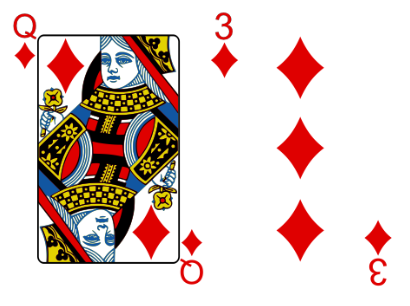
\includegraphics[width=0.2\textwidth, height=\textheight, keepaspectratio]{lilit.png}
			\end{center}
			She wonders how many more \textbf{diamonds} there are in the community cards.\pause
			
			Aram, on the other hand, has the following cards:
			\begin{center}
				
				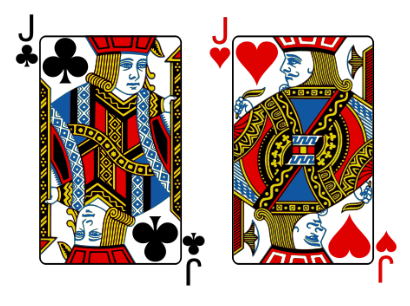
\includegraphics[width=0.2\textwidth, height=\textheight, keepaspectratio]{aram.png}
			\end{center}
			He is interested in the number of \textbf{jacks} among the community cards.\pause
			
			Both Lilit and Aram are interested in the same random process, yet different RVs. \textit{How much} are those RVs related?
			% \end{example}
	\end{frame}

		\begin{frame}{Covariance}
				\begin{block}{Definition}
						The \textbf{covariance} between random variables \( X \) and \( Y \) is defined by
						\[ \text{Cov}(X, Y) = \E\big((X - \E(X)(Y - \E(Y)\big) \]
						
					\end{block}\pause
				Note that the formula for covariance can be simplified to
				\[ \Cov(X, Y) = \E(XY) - \E(X)\E(Y) \]
%				
				\pause Covariance shows how much the linear growth of one RV is related to the linear growth of the other RV. It is very similar to the concept of dot product of the two vectors.
				
			\end{frame}
	
	% slide __: covariance
	\begin{frame}{Covariance}
		\begin{figure}
			\centering
			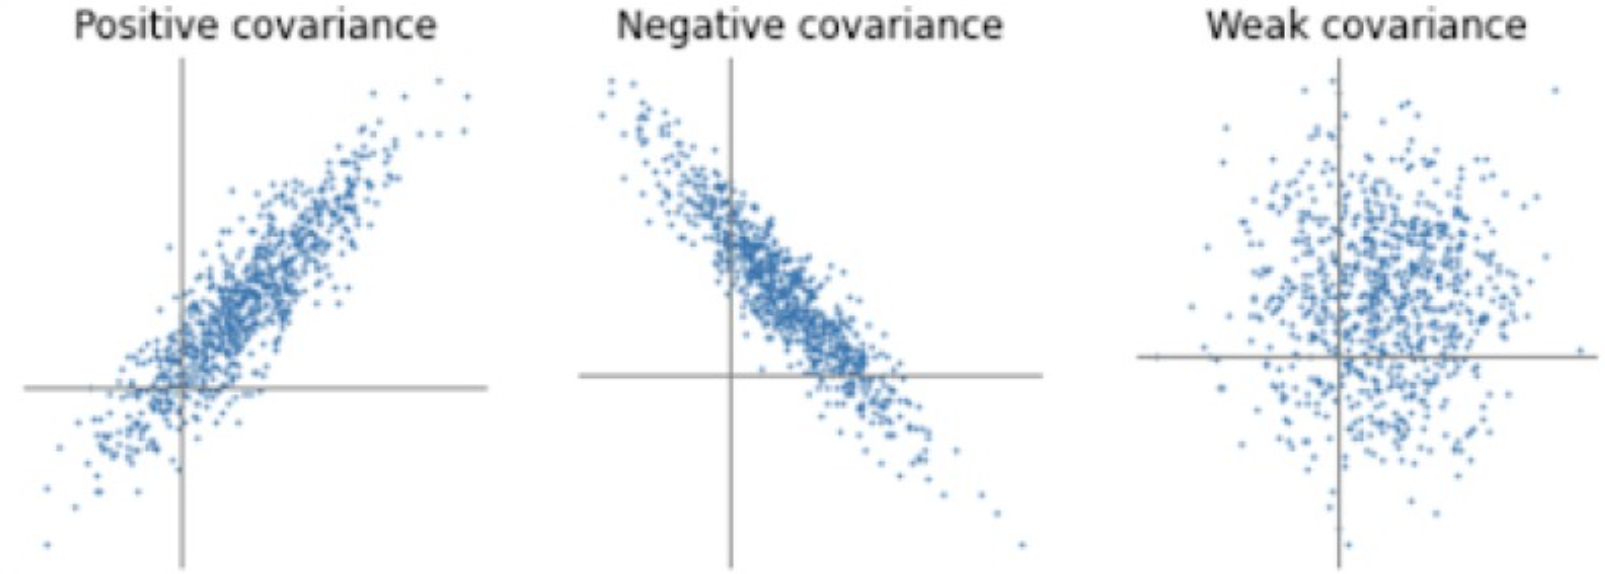
\includegraphics[width=0.9\linewidth]{screenshot001}
%			\caption{}
%			\label{fig:screenshot001}
		\end{figure}
		
	\end{frame}
	
	
	% slide __: covariance
	\begin{frame}{Covariance}
		\begin{block}{Properties}
			\begin{enumerate}[<+->]
				\item \( \text{Cov}(X, Y) = \text{Cov}(Y, X) \),
				\item \( \text{Cov}(X, X) = \text{Var}(X) \),
				\item  \( \text{Cov}(a \cdot X, Y) = a \cdot \text{Cov}(X, Y) \),
				\item  \(\displaystyle \text{Cov}\left( X_1+X_2, Y_1+Y_2\right) = \text{Cov}(X_1, Y_1) +\text{Cov}(X_1, Y_2) +\text{Cov}(X_2, Y_1) +\text{Cov}(X_2, Y_2) \),
				\item  \(\displaystyle \text{Var}\left(X_1+X_2\right) = \text{Var}(X_1)+\text{Var}(X_2)+2\cdot \text{Cov}(X_1, X_2) \),
				\item If $X$ and $Y$ are independent, $\text{Cov}(X, Y)=0$ (converse isn't true).
				
			\end{enumerate}
		\end{block}
		\pause 
		$\text{Cov}(X, Y)$ can be \textit{any} number (positive/negative, large/small, zero, etc). What if we want a normalized, universal method to measure the relatedness level of two RVs?
		
	\end{frame}
	
	% slide __: corr
	\begin{frame}{Correlation}
		
		\begin{block}{Definition}
			For two non-constant ($\text{Var}(X), \text{Var}(Y) \ne 0$) random variables \( X \) and \( Y \), the \textbf{correlation} (or \textbf{Pearson correlation coefficient}) between them is defined as:
			\[ \rho(X,Y)=\text{Corr}(X, Y) = \frac{\text{Cov}(X, Y)}{\sqrt{\text{Var}(X) \cdot \text{Var}(Y)}} \]
			
		\end{block}
		\pause
		\begin{block}{Properties}
			\begin{enumerate}
				\item \( \rho(X, Y) = \rho(Y, X) \),
				\item \( -1 \le \rho(X, Y) \leq 1 \),
				\item \( Y = aX + b \) for some constants \( a, b \) if and only if \( \rho(X, Y) = \pm 1 \).
			\end{enumerate}
		\end{block}
		
	\end{frame}
	
	% slide __: corr
	\begin{frame}{Correlation}
		\begin{figure}
			\centering
			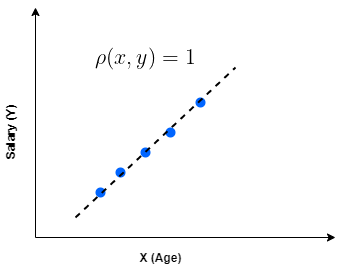
\includegraphics[width=0.3\linewidth]{screenshot002}
%%			\caption{}
%			\label{fig:screenshot002}
%		\end{figure}		\begin{figure}
%%			\centering
			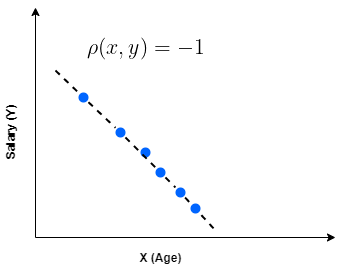
\includegraphics[width=0.3\linewidth]{screenshot003}
%%			\caption{}
%			\label{fig:screenshot003}
%		\end{figure}
%		\begin{figure}
%%			\centering
			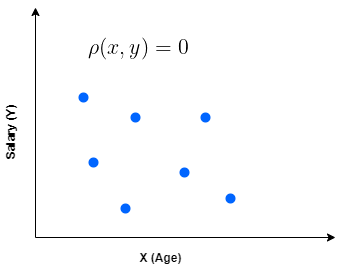
\includegraphics[width=0.3\linewidth]{screenshot004}
%			\caption{}
			\label{fig:screenshot004}
		\end{figure}
		\begin{figure}
			\centering
			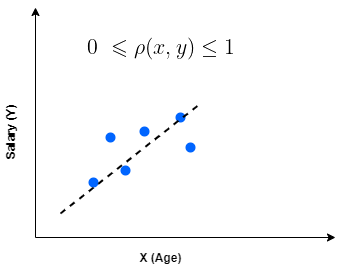
\includegraphics[width=0.3\linewidth]{0.33}
%			\caption{}
%			\label{fig:0}
%		\end{figure}
%		\begin{figure}
%%			\centering
			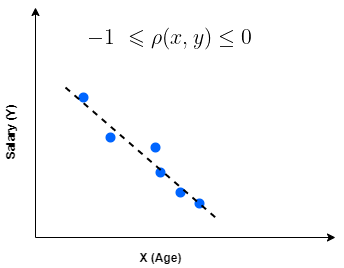
\includegraphics[width=0.3\linewidth]{0.34}
%			\caption{}
			\label{fig:0}
		\end{figure}
		
	\pause
 - \color{blue} \href{https://www.geogebra.org/m/w5q22bzu}{Play with this correlation visualization!}

	\end{frame}
	
	
	% slide 5
	\begin{frame}{Distributions}
		Very often in practice, many random variables share similar properties. In particular, the probabilities of their values seem to follow a common pattern, i.e. their CDFs (or PMFs/PDFs) are similar to each other:
		\begin{figure}
			\centering
			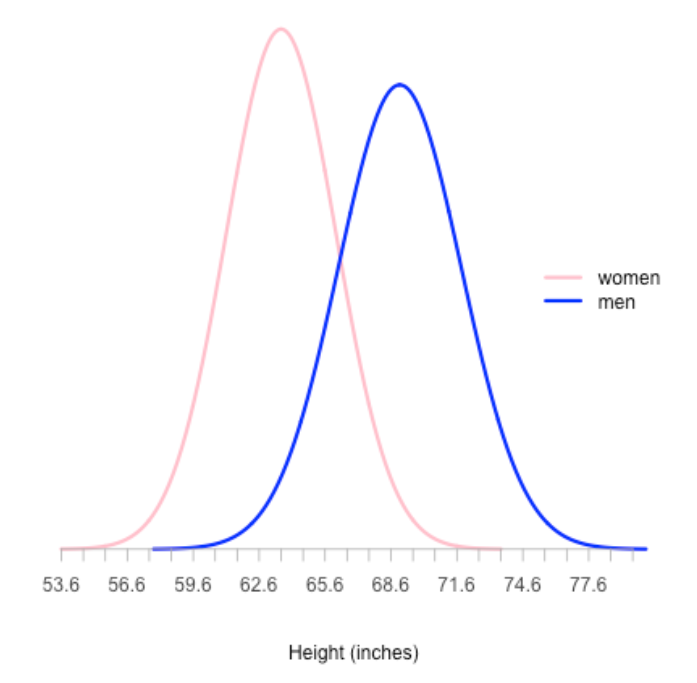
\includegraphics[width=0.45\linewidth]{0.35}
%			\caption{}
			\label{fig:0}
		\end{figure}
		\pause The way the values of an RV are distributed is called a \textit{distribution}.
		
		
	\end{frame}
	
	
	% slide 6: bern
	\begin{frame}{Bernoulli Distribution}
	Consider these situations:\pause
	\begin{itemize}[<+->]
\item You take a pass-fail exam. You either pass or fail.
\item You toss a coin. The outcome is either heads or tails.
\item A child is born. The gender at birth is either male or female.
	\end{itemize}
		
		\pause 
		\begin{block}{Definition}
			A random variable $X$ is said to be a \textbf{Bernoulli} random variable with parameter $p$, denoted by $X\sim Bernoulli(p)$, if it only takes two values and its PMF is given by:
			\begin{equation}
				\nonumber \PP(X=x) = \left\{
				\begin{array}{l l}
					p& \quad \text{ for } x=1\\
					1-p & \quad \text{ for } x=0\\
					0 & \quad \text{ otherwise}
				\end{array} \right.
			\end{equation}
			where $0<p<1$.
		\end{block}
		\pause 
%			\begin{block}{Definition}
					A series of $n$ independent experiments all following Bernoulli distribution $Bernoulli(p)$, is called \textbf{Bernoulli trials}.
%					(One such experiment is called a trial.)
%				\end{block}
	\end{frame}
	
	
	
	% slide 6: bern
	\begin{frame}{Bernoulli Distribution}
	\begin{figure}
		\centering
		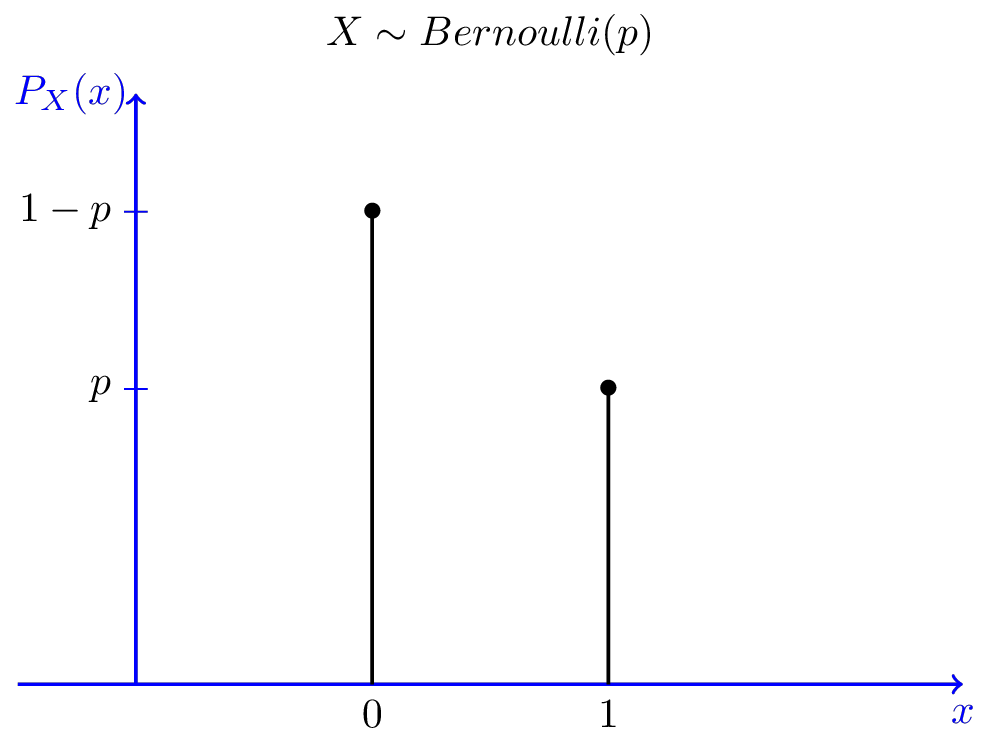
\includegraphics[width=0.6\linewidth]{0.36}
%		\caption{}
		\label{fig:0}
	\end{figure}
	\pause
%	\begin{block}{Definition}
%		A series of $n$ independent experiments all following Bernoulli distribution $Bernoulli(p)$, is called \textbf{Bernoulli trials}.
%	\end{block}
%	
If $X\sim Bernoulli(p)$,
\[ \E(X) = p,\qquad \Var(X)=p(1-p) \]
	\end{frame}
	
	
	% slide 6: geo
	\begin{frame}{Geometric Distribution}
		Suppose we have a coin with $\PP(\text{Heads})=p$ and we toss it until we observe the first Heads, after which we stop. We define $X$
		as the total number of coin tosses in this experiment. Then X
		is said to have \textit{geometric distribution} with parameter $p$. 
		\pause
		
		For any natural number $k\ge 1$:
		\[\PP(X=k)=(1-p)^{k-1} p\] \pause		\begin{block}{Definition}
		A random variable $X$ is said to be a \textbf{geometric} random variable with parameter $p$, denoted by $X\sim Geo(p)$, if its PMF is given by:
	\begin{equation}
		\nonumber \PP(X=k) = \left\{
		\begin{array}{l l}
			(1-p)^{k-1} p& \quad \text{ for } k=1,2,3,\dots\\
			0 & \quad \text{ otherwise}
		\end{array} \right.
	\end{equation}
	where $0<p<1$.
		\end{block}
  % \pause
		% In other words, if we repeat Bernoulli trials until the first success, we have geometric distribution.
		
	\end{frame}
	
	
	
	% slide 6: geo
	\begin{frame}{Geometric Distribution}
	\begin{figure}
		\centering
		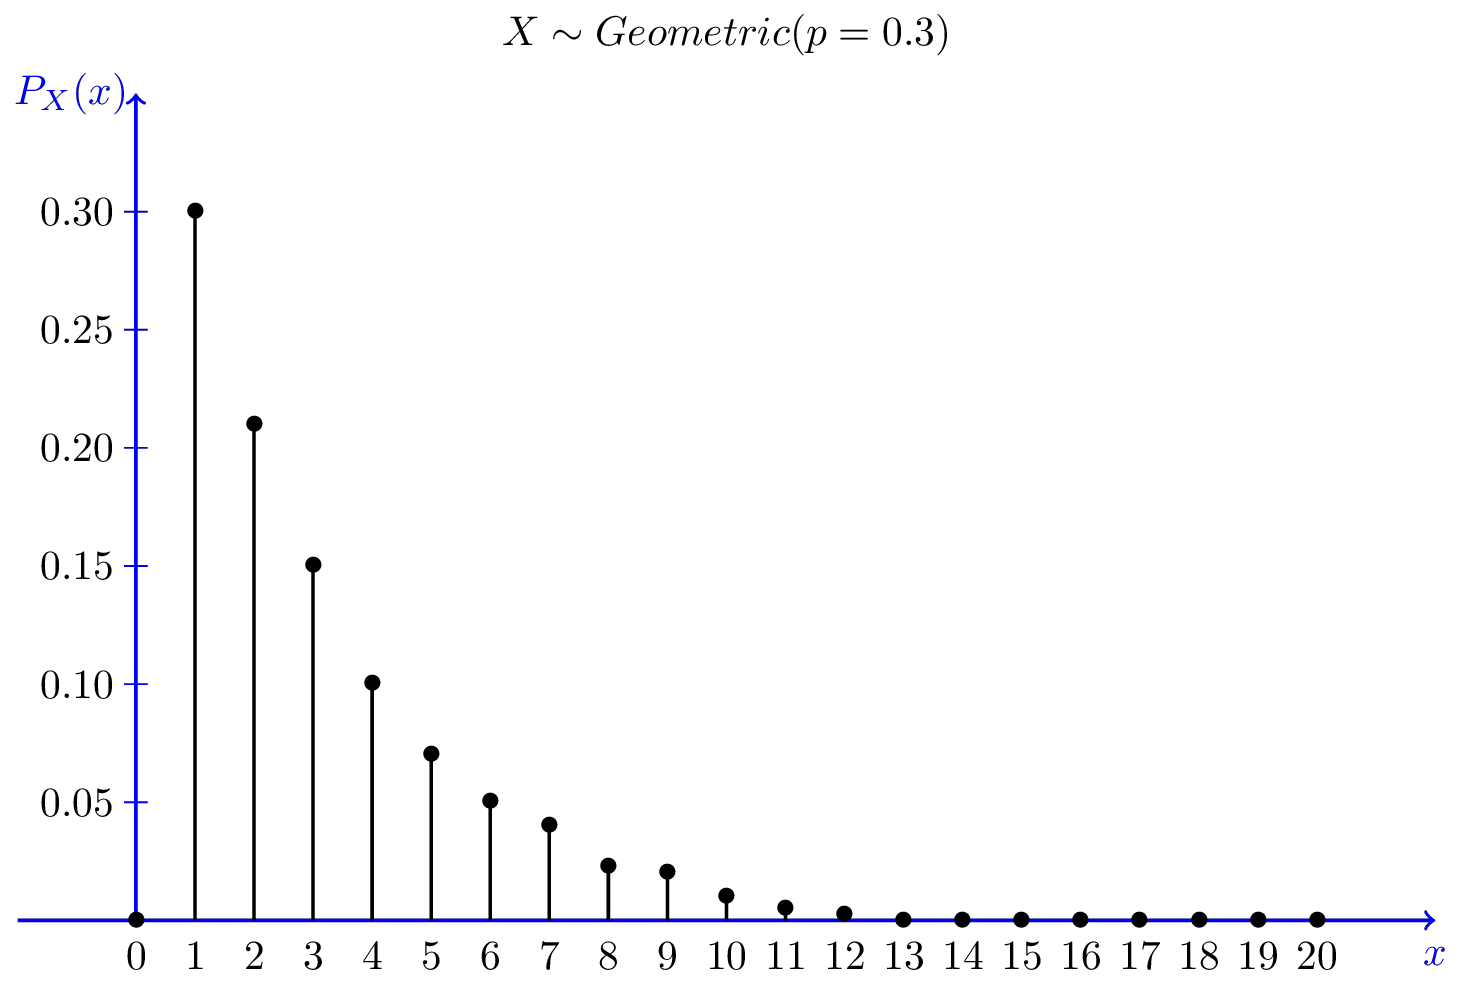
\includegraphics[width=0.6\linewidth]{0.37}
%		\caption{}
%		\label{fig:0}
	\end{figure}
	\pause
	If $X\sim Geo(p)$,
	\[ \E(X) = \frac{1}{p},\qquad \Var(X)=\frac{1-p}{p^2} \]
	
		
	\end{frame}
	
	
	
	% slide 7: binom
	\begin{frame}{Binomial Distribution}
		Suppose we have a coin with $\PP(\text{Heads})=p$ and we toss it $n$
		times. We define $X$ to be the total number of Heads observed. Then $X$ is said to have \textit{binomial distribution} with parameter $n$
		and $p$.
%		In other words, we repeat $n$ Bernoulli trials and want\pause
		
		\pause
		For any whole number $k\ge 0$:
		\[\PP(X=k)=C_n^k p^k(1-p)^{n-k}\]
		\pause
%		\paus
		\begin{block}{Definition}
			A random variable $X$ is said to be a \textbf{binomial} random variable with parameters $n$ and $p$, denoted by $X\sim B(n,p)$, if its PMF is given by:
			\begin{equation}
				\nonumber \PP(X=k) = \left\{
				\begin{array}{l l}
					C_n^k p^k(1-p)^{n-k}& \quad \text{ for } k=0,1,2,\dots\\
					0 & \quad \text{ otherwise}
				\end{array} \right.
			\end{equation}
			where $0<p<1$.
		\end{block}
		
	\end{frame}
		% slide 7:bin
	\begin{frame}{Binomial Distribution}
\begin{figure}
	\centering
%	\caption{}
	\label{fig:0}
	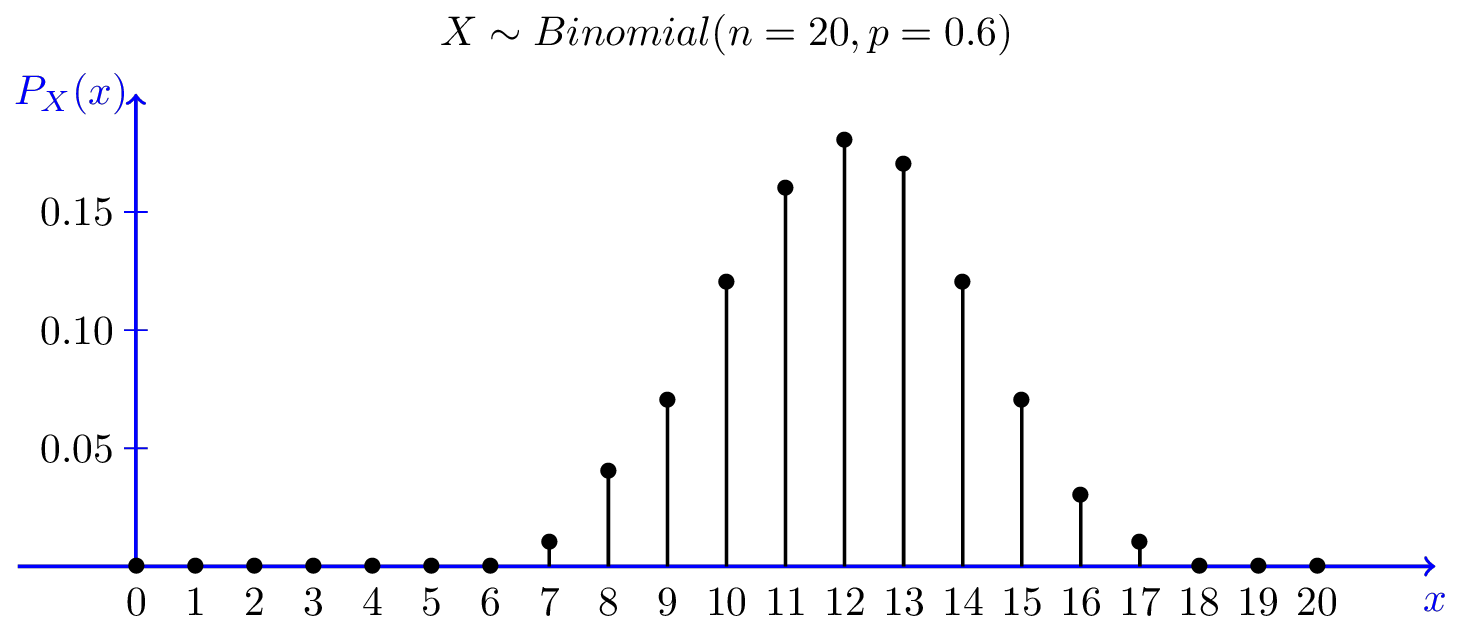
\includegraphics[width=0.6\linewidth]{0.38}
\end{figure}
		\pause
		If $X\sim B(n,p)$,
		\[ \E(X) = np,\qquad \Var(X)=np(1-p) \]
		
		
	\end{frame}
	
	
	
	% slide 8: pois
	\begin{frame}{Poisson Distribution}
		The Poisson distribution is one of the most widely used probability distributions. It is usually used in scenarios where we are counting the occurrences of certain events in an interval of time or space. In practice, it is often an approximation of a real-life random variable. \pause
		
		Suppose we are counting the number of customers who visit a certain store from 13:00 to 14:00. Based on data from previous days, we know that on average, $\lambda=15$ customers visit the store. \pause In practice, the number of customers tends to follow the following pattern:
		\pause
		%		\paus
		\begin{block}{Definition}
			A random variable $X$ is said to be a \textbf{Poisson} random variable with parameter $\lambda$, denoted by $X\sim Poisson(\lambda)$, if its PMF is given by:
			\begin{equation}
				\nonumber P_X(k) = \left\{
				\begin{array}{l l}
				\dfrac{\lambda^k}{k!}	e^{-\lambda} & \quad \text{for } k=0, 1, 2, \dots\\
					0 & \quad \text{otherwise}
				\end{array} \right.
			\end{equation}
%			where $0<p<1$.
		\end{block}
		
	\end{frame}
	% slide 8:pois
	\begin{frame}{Poisson Distribution}
\begin{figure}
	\centering
%	\caption{}
	\label{fig:0}
	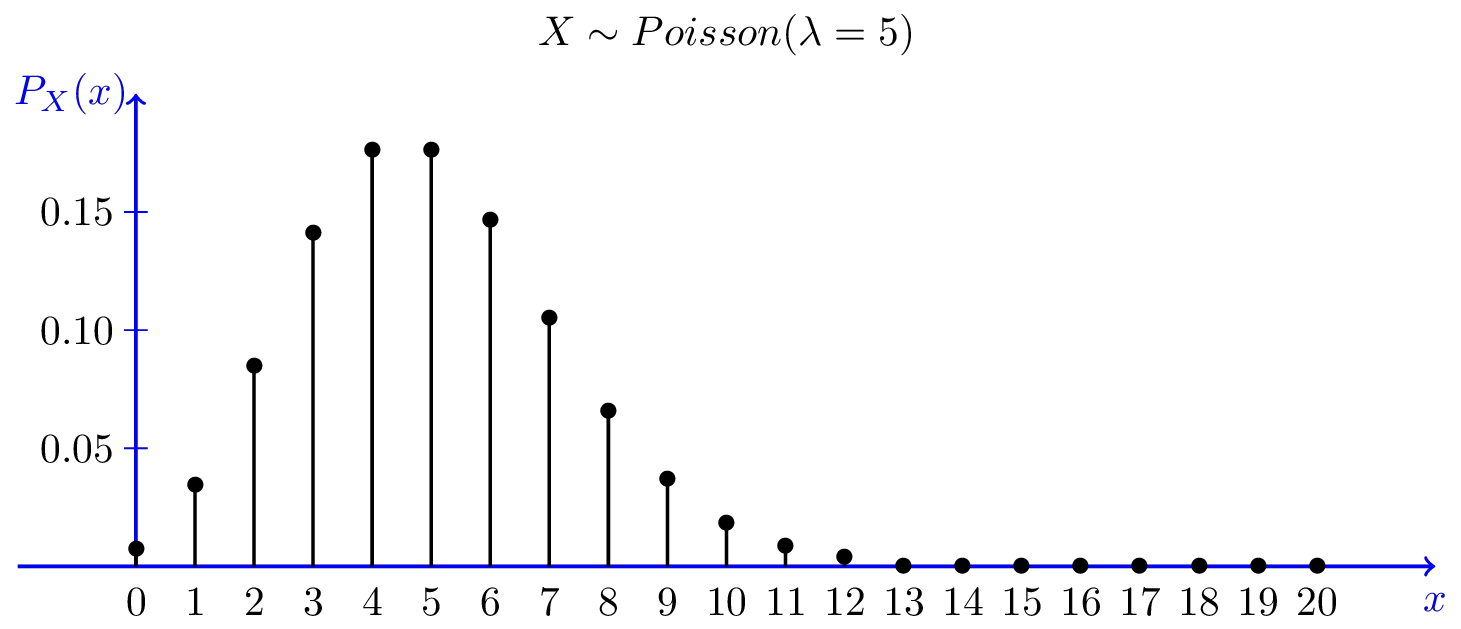
\includegraphics[width=0.6\linewidth]{0.39}
\end{figure}
		\pause
		If $X\sim Poisson(\lambda)$,
		\[ \E(X) = \lambda,\qquad \Var(X)=\lambda \]
		\pause
		\begin{block}{Remark}
		If $X\sim B(n, p)$, then
		\[\PP(X = k) \approx \frac{\lambda^k}{k!}e^{-\lambda},\qquad \text{where }\lambda = np\]
		\end{block}
		
	\end{frame}
	
	
	% slide 8: uni
	\begin{frame}{Uniform Distribution}
		So far, we have considered only discrete RVs. Let's observe some common distributions for continuous RVs.
		
		\pause
		If we pick a random number $X$ from a given interval, without any number being "more probable" than another, then $X$ is said to be \textit{uniformly} distributed.\pause
		%		\paus
		\begin{block}{Definition}
			A random variable $X$ is said to be a \textbf{uniform} random variable over the interval $[a,b]$, denoted by $X\sim U(a,b)$, if its PDF is given by:
			\begin{equation}
				\nonumber f(x) = \left\{
				\begin{array}{l l}
					\frac{1}{b-a} & \quad x\in (a,b)\\
					0 & \quad x\notin (a,b)
				\end{array} \right.
			\end{equation}
			%			where $0<p<1$.
		\end{block}\pause
		
		\begin{equation}
			\nonumber F(x) = \left\{
			\begin{array}{l l l}
				0 & \quad x \le a\\
				\frac{x-a}{b-a} & \quad a < x < b\\
				1 & \quad x \ge b
			\end{array} \right.
		\end{equation}
		
	\end{frame}
	\begin{frame}{Uniform Distribution}
		\begin{figure}
			\centering
			%	\caption{}
			\label{fig:0}
			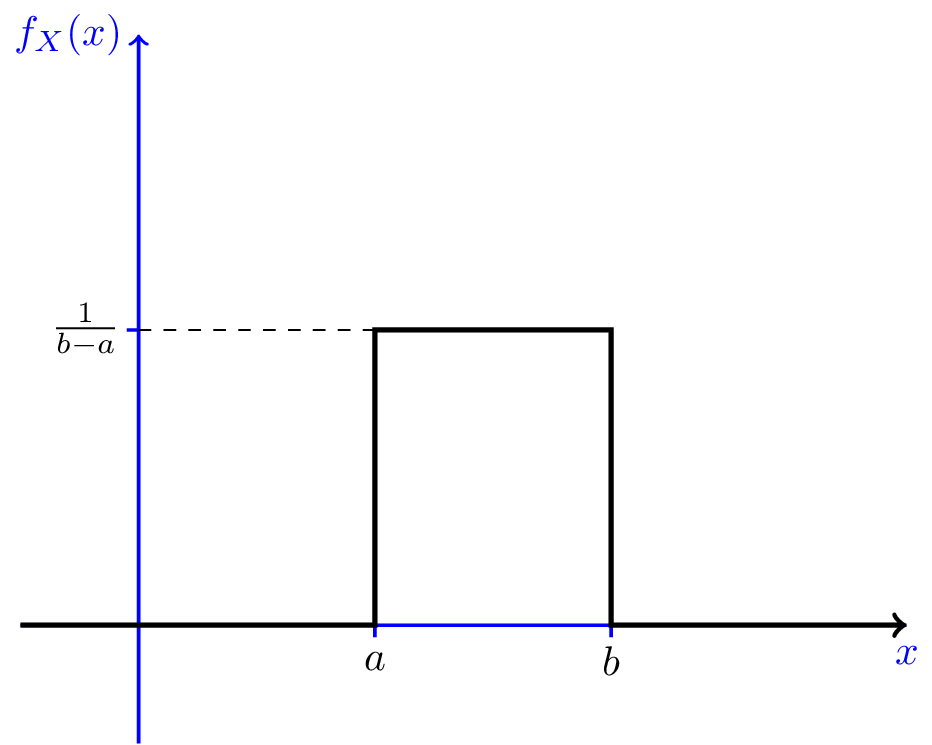
\includegraphics[width=0.6\linewidth]{ex_pdf}
		\end{figure}
		\pause
		If $X\sim U(a,b)$,
		\[ \E(X) = \frac{a+b}{2},\qquad \Var(X)=\frac{(b-a)^2}{12} \]
%		\end{block}
		
	\end{frame}
	
	
	
	% slide 8: uni
	\begin{frame}{Exponential Distribution}
		The \textit{exponential} distribution is the continuous analog of the geometric distribution. It is one of the widely used continuous distributions, and is often used to model the time elapsed between events.
		
		\pause
		
		%		\paus
		\begin{block}{Definition}
			A random variable $X$ is said to be a \textbf{exponential} random variable with parameter $\lambda>0$, denoted by $X\sim Exp(\lambda)$, if its PDF is given by:
		\begin{equation}
			\nonumber f_X(x) = \left\{
			\begin{array}{l l}
				\lambda e^{-\lambda x} & \quad x > 0\\
				0 & \quad \text{otherwise}
			\end{array} \right.
		\end{equation}
			%			where $0<p<1$.
		\end{block}\pause
		
		\begin{block}{Remark}
		If $X\sim Exp(\lambda)$, then $X$ is a \textbf{memoryless} random variable, that is
		\[\PP(X > x+a \hspace{5pt} | \hspace{5pt} X > a)=\PP(X > x), \hspace{10pt} \text{ for }a,x \geq 0.\]
		\end{block}
		
	\end{frame}
	\begin{frame}{Exponential Distribution}
\begin{figure}
	\centering
%	\caption{}
	\label{fig:0}
	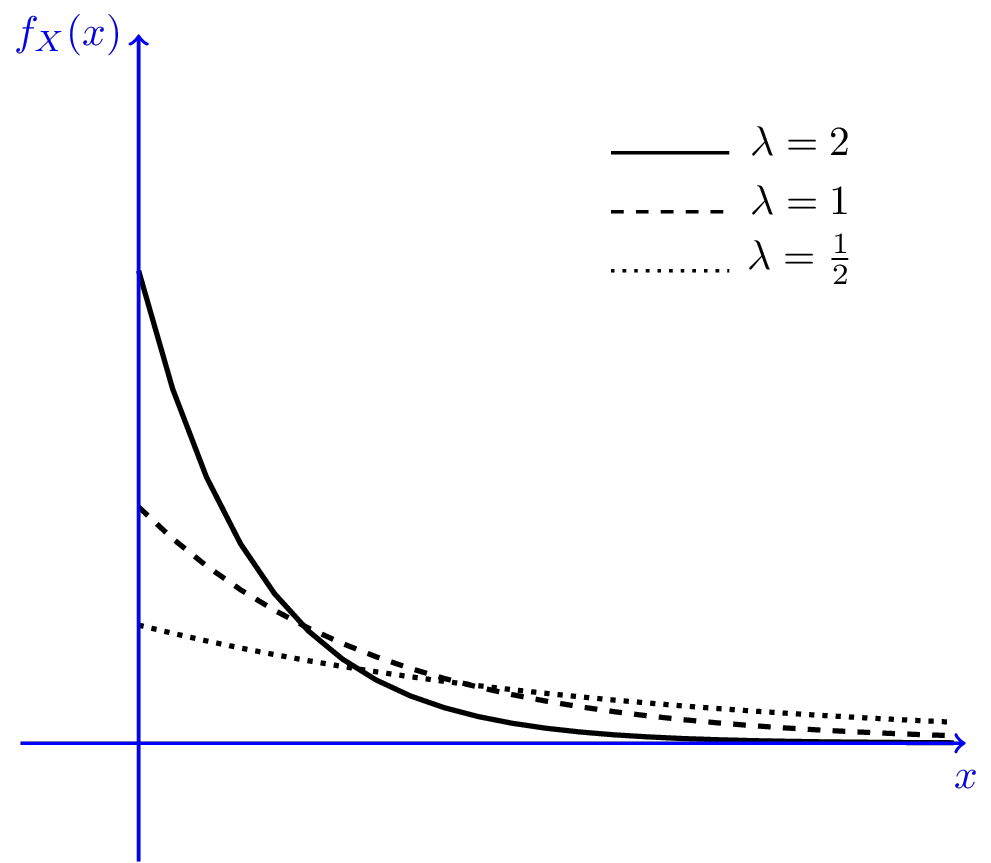
\includegraphics[width=0.6\linewidth]{0.40}
\end{figure}
		\pause
		If $X\sim Exp(\lambda)$,
		\[ \E(X) = \frac{1}{\lambda},\qquad \Var(X)=\frac{1}{\lambda^2} \]
		%		\end{block}
	
	\end{frame}
	
	
	
	
	% slide 8: uni
	\begin{frame}{Normal Distribution}
		The \textit{normal} distribution is by far the most important probability distribution. \pause
		
		One of the main reasons for that is that if you add a large number of random variables, the distribution of the sum will be approximately normal under certain conditions. In real life, many RVs can be expressed as the sum of a large number of random variables, and their distribution is normal. 
		
		\pause
		
		\begin{block}{Definition}
		A random variable $X$ is said to be a \textbf{normal} random variable with mean $\mu$ and variance $\sigma^2$, denoted by $X\sim N(\mu, \sigma^2)$, if its PDF is given by:
		\begin{equation}
			\nonumber f_X(x) = \frac{1}{ \sqrt{2 \pi}\sigma} e^{-\frac{(x-\mu)^2}{2\sigma^2}},\qquad x\in\R
		\end{equation}
		%			where $0<p<1$.
	\end{block}
	\end{frame}
	\begin{frame}{Normal Distribution}
%		\begin{figure}
%			\centering
%			%	\caption{}
%			\label{fig:0}
%			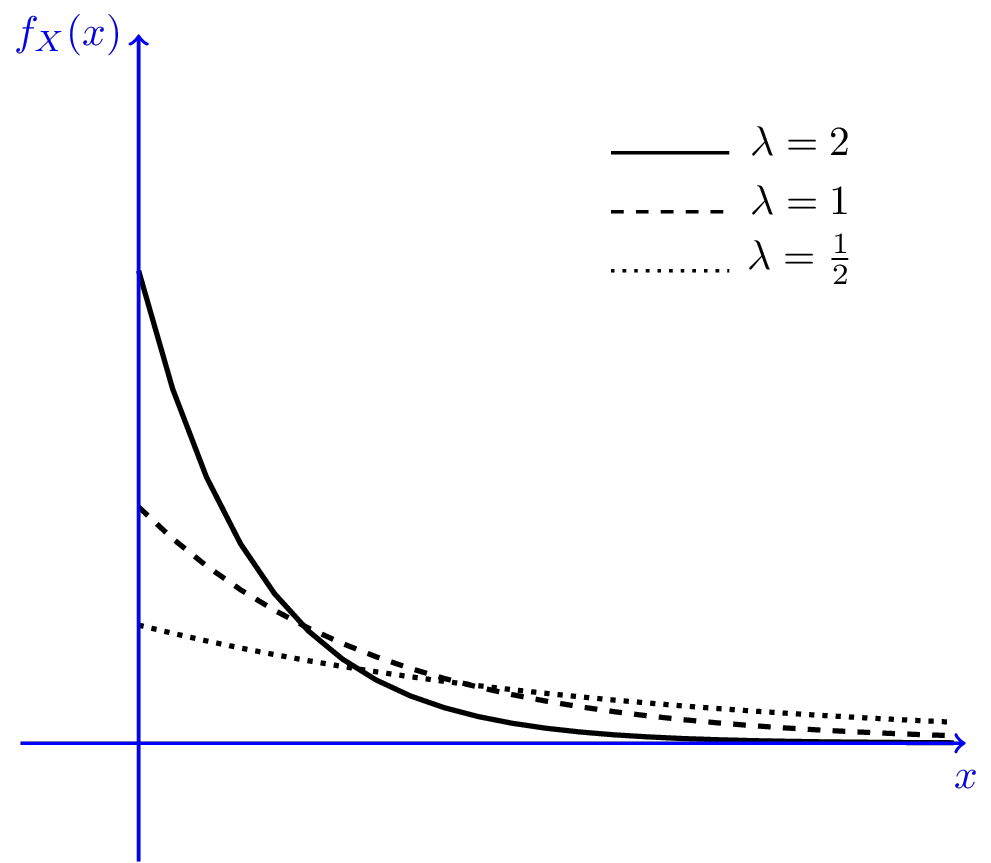
\includegraphics[width=0.6\linewidth]{0.40}
%		\end{figure}
%		\pause
%		If $X\sim Exp(\lambda)$,
%		\[ \E(X) = \frac{1}{\lambda},\qquad \Var(X)=\frac{1}{\lambda^2} \]
%		%		\end{block}
\begin{figure}
	\centering
	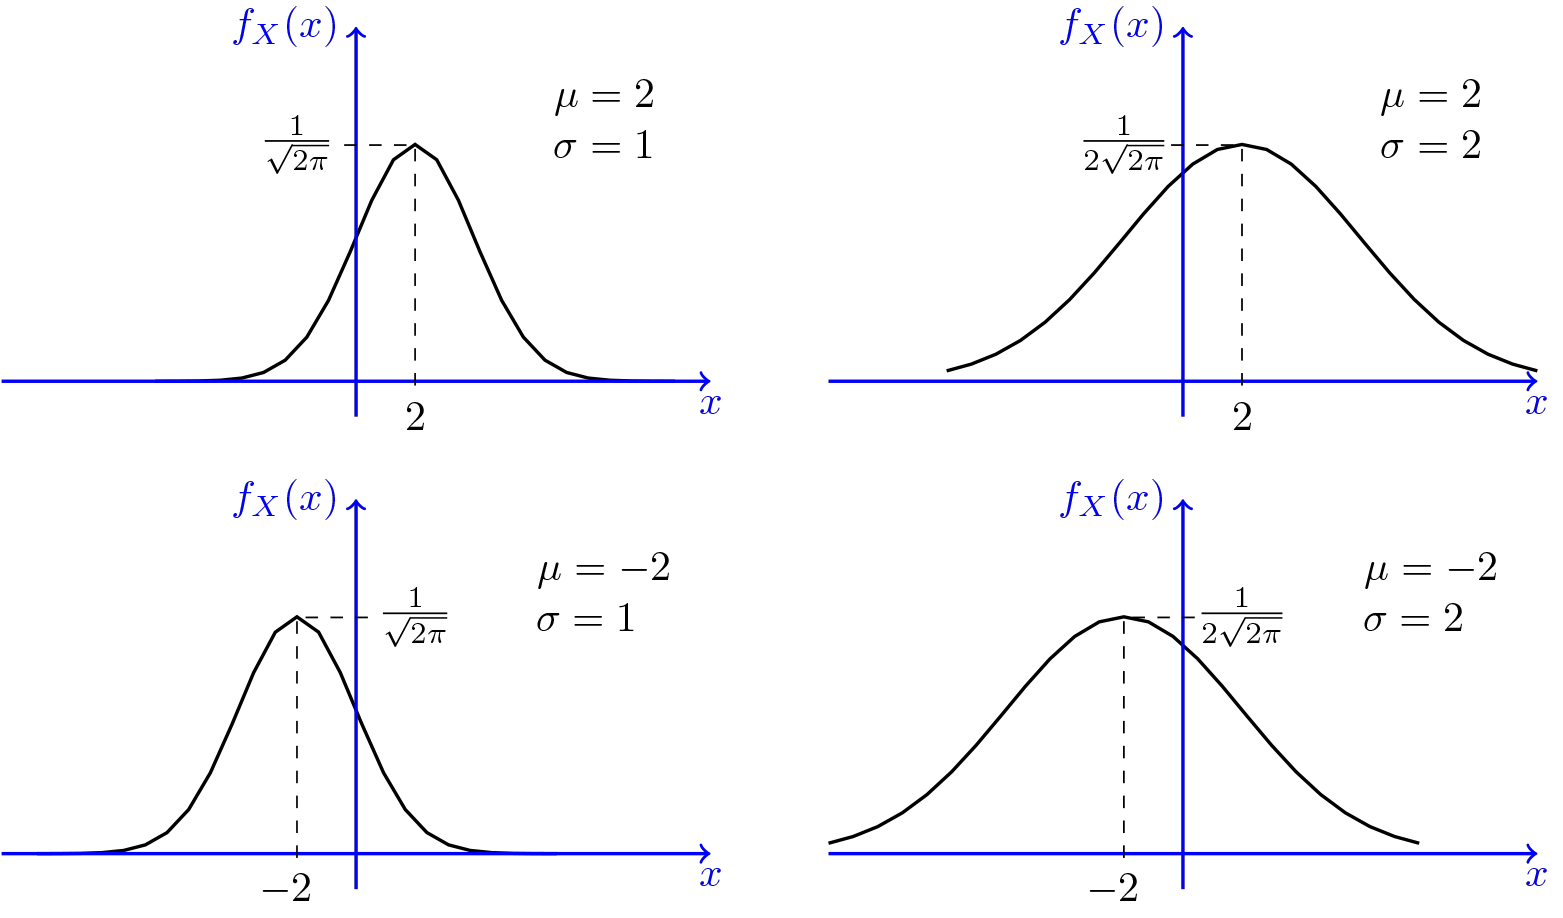
\includegraphics[width=1\linewidth]{0.42}
%	\caption{}
	\label{fig:0}
\end{figure}

	
	\end{frame}
	
	
	
\end{document}
